\documentclass{article}

% Language setting
% Replace `english' with e.g. `spanish' to change the document language
\usepackage[english]{babel}
\usepackage{float}
% Set page size and margins
% Replace `letterpaper' with `a4paper' for UK/EU standard size
\usepackage[letterpaper,top=2cm,bottom=2cm,left=3cm,right=3cm,marginparwidth=1.75cm]{geometry}

% Useful packages
\usepackage{amsmath}
\usepackage{graphicx}
\usepackage{amssymb}
\usepackage{stmaryrd}
\usepackage[colorlinks=true, allcolors=blue]{hyperref}
\graphicspath{{images/}}
\title{\Huge{Calcul Scientifique Numérique\\\\Projet 2:\\Approximation d'un problème de frontière libre par méthode analytique}}
\author{\large{Lucien Gontier \& Pierre Bichon } \\ \\ \large{M2MACS} \\  \large{2023-2024}}

\begin{document}
\maketitle
\vspace*{25\baselineskip}
\begin{figure}[h]
\centering
\center{
\includegraphics[width=0.5\linewidth]{Images/logo.png}}
\end{figure}
\newpage

\section{Introduction}

Dans ce projet, nous essaierons d'implémenter une méthode pour approcher la solution $T$ du problème suivant:
\[
\left \{
\begin{align*}
    \Delta T(x;y)&=0&\text{    dans }\Omega\\
    \frac{\partial T}{\partial x}(x;y)&=0&\text{   sur }\Gamma_1\cup\Gamma_2\\
    T(x;y)&=T_0(x)&\text{   sur }\Gamma\\
    -\frac{\partial T}{\partial y}(x;0)&=q_0(x)&\text{   sur }\Gamma_0\\
    T(x;0)&=f_0(x)&\text{   sur }\Gamma_0
\end{align*}
\]
où $\Omega\subset\mathbb{R}^2$, $\partial\Omega =\Gamma\cup\Gamma_0\cup\Gamma_1\cup\Gamma_2$ et où $\Gamma_0 =\lbrack 0;L\rbrack\times\{ 0\}$, $\Gamma =\{(x;y)\in\lbrack 0;L\rbrack\times\mathbb{R}\ \lvert \ y=f(x)\}$, $\Gamma_1=\{ 0\}\times\lbrack 0;f(0)\rbrack$ et $\Gamma_2=\{ L\}\times\lbrack 0;f(L)\rbrack$ avec $L\in\mathbb{R}_+^*$ et $f\in\mathcal{C}^0(\Gamma_0)$, une fonction à déterminer.
\\
\\
On note que la grande difficulté pour résoudre ce problème réside dans le fait que l'on ne connaît pas le bord $\Gamma$. Pour remédier à ce problème, on se propose d'étendre notre espace $\Omega$ de la solution en un espace rectangulaire $D\subset\mathbb{R}^2$ contenant $\Omega$. On se ramène alors à la résolution d'un nouveau problème:
\[
\left \{
\begin{align*}
    \Delta\tilde{T}(x;y)&=0&\text{    dans }D\\
    \frac{\partial\tilde{T}}{\partial x}(x;y)&=0&\text{   sur }\tilde{\Gamma_1}\cup\tilde{\Gamma_2}\\
    -\frac{\partial\tilde{T}}{\partial y}(x;0)&=q_0(x)&\text{   sur }\Gamma_0\\
    \tilde{T}(x;0)&=f_0(x)&\text{   sur }\Gamma_0\\
    \tilde{T}(x;H)&=f_3(x)&\text{   sur }\Gamma_3
\end{align}
\]
Où $\partial D=\Gamma_0\cup\tilde{\Gamma_1}\cup\tilde{\Gamma_2}\cup\Gamma_3$ avec $\tilde{\Gamma_1}=\{ 0\}\times\lbrack 0;H\rbrack$, $\tilde{\Gamma_2}=\{ L\}\times\lbrack 0;H\rbrack$ et $\Gamma_3=\lbrack 0;L\rbrack\times\{ H\}$ et $H\in\mathbb{R}_+^*$ et $f_3:\Gamma_3\to\mathbb{R}$ est une fonction inconnue.
\\
\\
Nous allons à présent tâcher de résoudre ce problème sur $D$ pour ensuite résoudre notre prolème initial sur $\Omega$. On note qu'avec le problème sur $D$, nous perdons la condition "$T(x;y)=T_0(x)$" sur $\Gamma$ car $\Gamma$ n'est plus un bord de l'espace de la solution. Par ailleurs, on a "remplacer" cette condition par la condition inconnue "$\tilde{T}(x;H)=f_3(x)$" sur $\Gamma_3$. Cependant, pour résoudre le problème sur $D$, on a besoin d'appliquer des contraintes connues. C'est pourquoi, nous allons tenter de "recréer" notre condition sur le bord $\Gamma$ de $\Omega$ en introduisant un espace $\tilde{\Gamma}:=\{ (x;y)\in D \ | \ \tilde{T}(x;y)=T_0(x)\}\subset D$. On définit également l'espace $\tilde{\Omega}\subset D$, délimité par $\Gamma_0$, $\{ 0\}\times\lbrack 0;a\rbrack$, $\{ L\}\times\lbrack 0;b\rbrack$ et $\tilde{\Gamma}$ avec $a:=T_0(0)$ et $b:=T_0(L)$.
\\
On trouve ensuite que la restriction de $\tilde{T}$ à $\tilde{\Omega}$ n'est autre que la solution de notre problème initial sur $\tilde{\Omega}$ et du résultat d'unicité $\tilde{\Gamma}=\Gamma$.
\\
On peut donc commencer à chercher une solution de notre équation sur $\Omega$ en résolvant notre équation sur $D$.
\\
Pour cela, on utilise une méthode de résolution par séparation de variable. On suppose alors qu'il existe $X:\lbrack 0;L\rbrack\to\mathbb{R}$ et $Y:\lbrack 0;H\rbrack\to\mathbb{R}$ telles que pour tout $(x;y)\in D$, on ai:
\[
\tilde{T}(x;y)=X(x)Y(y)
\]
Alors, partant de cette hypothèse, on peut établir que l'équation sur $D$:
\[
\Delta T(x;y)=0
\]
revient à
\[
Y(y)X''(x)+X(x)Y''(y)=0
\]
Soit, en supposant que $\forall x\in\lbrack 0;L\rbrack, X(x)\neq 0$ et $\forall y\in\lbrack 0;H\rbrack, Y(y)\neq 0$:
\[
\frac{X''(x)}{X(x)}=\frac{-Y''(y)}{Y(y)}
\]
Comme on a cette équation pour tout $(x;y)\in D$, alors il existe $K\in\mathbb{R}$ telle que:
\[
\left\{
\begin{align}
    \frac{X''(x)}{X(x)}&=K\\
    \frac{Y''(y)}{Y(y)}&=-K
\end{align}
\]
On peut alors résoudre ces deux équations différentielles du second ordre. On obtient alors la solution suivante:
\[
\tilde{T}(x;y)=A_0+B_0 y+\sum_{m=1}^{\infty}\left( A_me^{\frac{m\pi}{L}y}+B_me^{\frac{-m\pi}{L}y}\right)\cos\left(\frac{m\pi}{L}x\right)
\]
avec:
\[
\begin{enumerate}
    \item A_0=\frac{1}{L}\int_0^Lf_0(x)dx\\
    \item B_0=\frac{1}{HL}\int_0^Lf_3(x)-f_0(x)dx\\
    \item A_m=\frac{1}{L\sinh\left(\frac{m\pi}{L}H\right)}\int_0^L\left( f_3(x)-e^{\frac{-m\pi}{L}H}f_0(x)\right) \cos\left(\frac{m\pi}{L}x\right)dx\\
    \item B_m=\frac{1}{L\sinh\left(\frac{m\pi}{L}H\right)}\int_0^L\left( e^{\frac{m\pi}{L}H}f_0(x)-f_3(x)\right) \cos\left(\frac{m\pi}{L}x\right)dx\\
\end{enumerate}
\]
On souhaîte maintenant déterminer la fonction $f_3$ telle que l'équation ci-dessus soit vraie. Pour cela, on a besoin d'appliquer la contrainte $\frac{\partial\tilde{T}}{\partial y}(x;0)=-q_0(x)$ que l'on a donnée précédemment. On a alors:
\[
\frac{\partial\tilde{T}}{\partial y}(x;0)=-q_0(x)
\]
$\Longleftrightarrow$
\[
B_0+\sum_{m=1}^{\infty}\frac{m\pi}{L}\left( A_me^{\frac{m\pi}{L}0}-B_me^{\frac{-m\pi}{L}0}\right)=-q_0(x)
\]
$\Longleftrightarrow$
\[
B_0+\sum_{m=1}^{\infty}\frac{m\pi}{L}\left( A_m-B_m\right)=-q_0(x)
\]
Ce qui équivaut après quelques calcul à:
\[
\begin{equation}
    h(x)=\int_0^Lk(x;t)f_3(t)dt
\end{equation}
\]
avec
\[
h(x)=-q_0(x)+\frac{1}{HL}\int_0^Lf_0(t)dt+\frac{2\pi}{L^2}\sum_{m=1}^{\infty}\frac{m\cos \left(\frac{m\pi x}{L}\right)\cosh\left(\frac{m\pi H}{L}\right)}{\sinh\left(\frac{m\pi H}{L}\right)}\int_0^Lf_0(t)\cos\left(\frac{m\pi t}{L}\right)dt
\]
et la fonction noyau $k$ donnée par 
\[
k(x;t)=\frac{1}{HL}+\frac{2\pi}{L^2}\sum_{m=1}^\infty\frac{m\cos \left(\frac{m\pi x}{L}\right)\cos\left(\frac{m\pi t}{L}\right)}{\sinh\left(\frac{m\pi H}{L}\right)}
\]
Or on rencontre ici un nouveau problème; en effet, l'équation (1) ci-dessus n'est pas résolvable de façon exacte. On souhaîte donc trouver une approximation de $f_3$. Pour cela, on introduit un $\alpha\neq 0$ que l'on supposera très proche de 0, et on résout:
\[
\begin{equation}
    h(x)=\alpha f_3(x)+\int_0^Lk(x;t)f_3(t)dt
\end{equation}
\]
Cependant, à nouveau, on ne peut pas obtenir de formulation exacte de $f_3$ avec cette équation. L'enjeu de ce projet sera donc de trouver des méthodes permettant de calculer une approximation $f_3^\alpha$ de la solution $f_3$
\section{Résolution du problème}
Pour résoudre ce problème, on commence par remarquer que notre dernière équation est équivalente à celle ci-dessous
\[
$$f_3(x)=\frac{h(x)}{\alpha}-\frac{1}{\alpha}\int_0^L k(x,t)f_3(t)dt$$
\]
En effet, on sait que $\alpha>0$.
Tout l'enjeu est donc le calcul du $f_3$, pour cela nous l'avons approximé par trois méthodes différentes.\\
\subsection{Méthode de décomposition d'Adomain}
La méthode de Adomain consiste à poser:
$$f_3(x)=u(x)=\sum_{n=0}^{\infty}u_n(x)$$
avec les $u_n$ définie par:
$$
\left\{
    \begin{array}{ll}
        u_0(x) &= \frac{h(x)}{\alpha} \neq 0 \\
         u_{n+1} &= -\frac{1}{\alpha}\displaystyle\int_{0}^{L}k(x,t)u_n(t)dt
    \end{array}
\right.
$$

\subsubsection{Méthode de décomposition d'Adomain v1}
Dans un premier temps on va utiliser cette méthode pour trouver une approximation numérique de $f_3$. Si on rentre dans la partie numérique on se rend rapidement compte que le schéma requiert des appels récursifs à notre fonction Un, cependant, lors de l'implémentation dès que nous montions au dessus de n=2, nous nous retrouvions avec un problème de mémoire. \\
Nous avons donc un autre point de vue, en effet, numériquement, la résolution d'une intégrale ne se fait pas sur une fonction, mais sur un vecteur de valeur de cette fonction. \\
Notre méthode de résolution de Gauss Legendre prend N points, nous avons donc $\forall n\geq 1$ :
$$U_n(x)\approx-\frac{1}{\alpha}\displaystyle\sum_{i=0}^{N-1} k\left(x,Xbis[i]\right)U_{n-1}\left(Xbis[i]\right)\omega[i]$$
avec les Xbis[i] les N points de notre méthode de Gauss legendre après changement de variables, et w[i] les poids associés.\\
\\
Donc on pose $Un[i]=U_{n-1}\left(Xbis[i]\right)$, que l'on viendra recalculer à chaque itération.\\
Et on crée la fonction GL2(tab\_f,a,b,m) qui renvoie, avec tab\_f la fonction f prise aux valeur de Xbis:
$$\displaystyle\sum_{i=0}^{N-1} \omega[i]tab\_f[i]cos(\frac{m\pi}{L}Xbis[i])\approx \displaystyle\int_a^bf(x)cos(\frac{m\pi}{L}x)dx$$
(L'entier m, permettant de d'intégrer la fonction contre $cos(\frac{m\pi}{L}x)$, nous est très utile, car ce genre de situation revient beaucoup dans ce projet.)
\\
De plus comme :
$$k(x,t)=\frac{1}{HL} +\frac{2\pi}{L^{2}}\sum_{m=1}^{\infty}\frac{m }{\sinh(\frac{m\pi}{L}H)}\cos(\frac{m\pi}{L}x)\cos(\frac{m\pi }{L}t) $$
on a :

\begin{align*}
\displaystyle\int_0^L k(x,t)U_n(t)dt &=\displaystyle\int_0^L \frac{1}{HL}U_n(t)dt +\displaystyle\int_0^L U_n(t)\sum_{m=1}^{\infty}\frac{m }{\sinh(\frac{m\pi}{L}H)}\cos(\frac{m\pi}{L}x)\cos(\frac{m\pi }{L}t)dt \\
&=\displaystyle\int_0^L \frac{1}{HL}U_n(t)dt +\sum_{m=1}^{\infty}\frac{m }{\sinh(\frac{m\pi}{L}H)}\cos(\frac{m\pi}{L}x)\displaystyle\int_0^L U_n(t)\cos(\frac{m\pi }{L}t)dt 
\end{align*}
Ce qui numériquement nous fait, avec $U_n$ le vecteur des valeurs de la fonction $U_n$ évalué aux N points de Gauss Legendre :
$$U_{n+1}(x)=-\frac{1}{\alpha}\left( \frac{1}{HL}GL2(U_n,0,L,0) + \displaystyle\sum_{m=1}^{N1}\frac{m }{\sinh(\frac{m\pi}{L}H)}\cos(\frac{m\pi}{L}x)GL2(U_n,0,L,m)\right)$$
Et voilà, maintenant, à chaque itération de boucle, il nous reste à calculer les N points de $U_n[i]$ qui sont les $U_n(Xbis[i])$ pour pouvoir l'utiliser à l'itération suivante, et le point $U_n(x)$ que nous ajouterons à $\displaystyle\sum_{k=0}^{n-1}U_k(x)$, pour obtenir $U(x)$ après le nombre d'itérations souhaités.
\\
\\
On peut alors appliquer la méthode et on obtient alors:
%Mettre une capture d'écran du terminal
\[
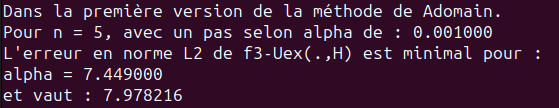
\includegraphics[scale=0.7]{Images/Capture d’écran du 2023-11-27 21-00-56.png}
\]
On en déduit que la méthode implentée fonctionne relativement. En effet, notre erreur semble relativement stable (elle est quand même d'ordre $10^0$).\\
On souhaîte à présent visualiser l'évolution de l'erreur selon $\alpha$ afin d'observer l'allure de la courbe.
\[
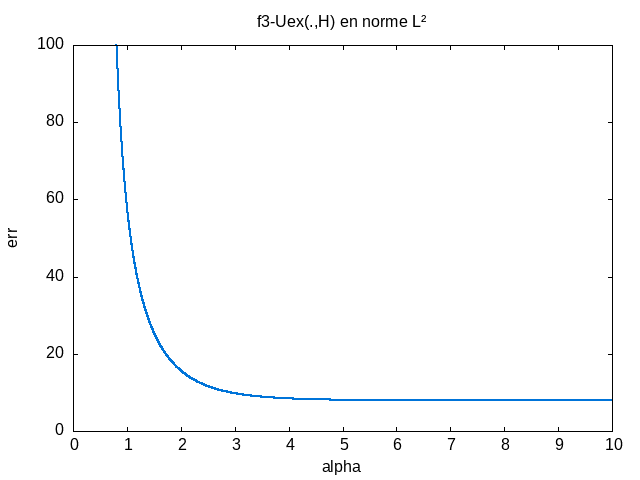
\includegraphics[scale=0.8]{Images/T_err_alpha_adov1.png}
\]
\[
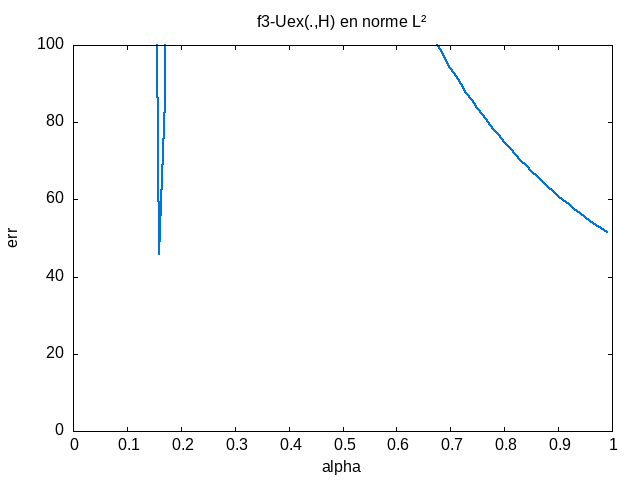
\includegraphics[scale=0.8]{Images/T_err_alpha_adov1_zoom.png}
\]
On a observé que l'erreur tendait vers $+\infty$ lorsque $\alpha \to 0$ et on ne pouvait donc pas visualiser correctrement la courbe des erreurs car lorsque $\alpha$ grandit, l'erreur reste assez négligeable par rapport aux valeurs de l'erreur quand $\alpha$ est proche de 0. C'est pourquoi nous avons restreint le graphique aux erreurs inférieures ou égales à 100 pour des valeurs de $\alpha$ comprises entre 0 et 1. On obtient ainsi le graphe ci-dessus.\\
\\
Concernant l'analyse de ce graphe, nous pouvons dire que l'erreur est très instable pour $\alpha\in\rbrack 0,1\rbrack$. En effet, lorsque $alpha$ est très proche de 0, on observe une erreur extrêmement grande, comme nous l'avons dit précédemment. On observe ensuite un pic dont nous n'avons pas trouvé de réelle explication en $\alpaha=0,18$ (on note quand même que pour ce $\alpha$, l'erreur reste de l'ordre de $10^1$), avant que l'erreur ne réexplose. A partir de $\alpha=0,35$, on observe une nouvelle décroissance de l'erreur qui se stabilise aux alentours de $\alpha=2$ jusqu'à ce qu'elle recroisse légèrement à partir de $\alpha=7,449$.\\
\\
De ce schéma, nous déduisons que notre méthode admet des problèmes au niveau des approxiomations numériques lorsque $\alpha$ est proche de 0. La stabilité de la méthode à partir de $\alpha=2$ nous laisse pourtant croire que notre méthode fonctionne relativement pour tout $\alpha\geq 2$. On garde cependant à l'esprit que notre erreur reste de l'ordre de $10^0$ en ces valeurs de $\alpha$.\\
\\
Nous allons maintenant nous interresser au tracé de $f_3^\alpha$ calculée par la méthode d'Adomain.\\
Voici la courbe de la solution calculée $f_3^\alpha$:


\begin{figure}{H}
    \centering
    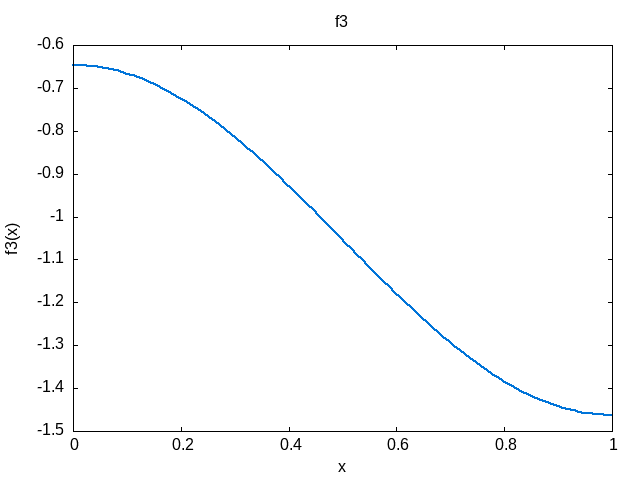
\includegraphics[scale=0.8]{newImages/f3_adov1.png}
    \caption{tracé de f3 pour la première version de Adomain}
    \label{fig:enter-label}
\end{figure}

\begin{figure}{H}
    \centering
    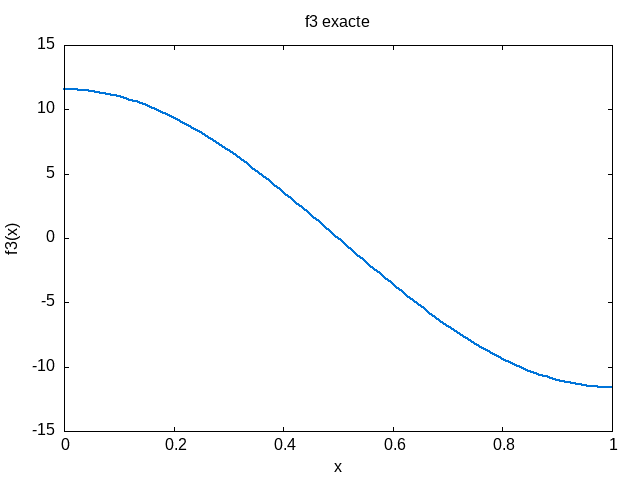
\includegraphics[scale=0.8]{newImages/f3_ex.png}
    \caption{tracé de f3 exacte}
    \label{fig:enter-label}
\end{figure}

Et 
On observe alors qu'en terme d'allure, notre $f_3^\alpha$ calculée par la méthode d'Adomain ressemble beaucoup à la courbe de notre $f_3$ attendue. La différence réside cependant dans les échelles. En effet, lorsque l'on s'interresse à l'échelle, on voit bien que la courbe de $f_3^\alpha$ a beaucoup moins d'amplitude que celle de $f_3$. En effet sur $\lbrack 0,1\rbrack$, la courbe de $f_3^\alpha$ peut être délimitée par -1,5 et -0,6, tandis que la courbe de $f_3$ est, elle, délimitée par -15 et 15. Mis à part ce problème d'échelle, on voit que la courbe de $f_3^\alpha$ reste plus ou moins centrée en -1, tout comme le courbe de $f_3$. On en déduit alors que la méthode d'Adomain a une fâcheuse tendance à afaisser la courbe lorsque cette dernière présente des variations trop grandes (en effet, ici, $f_3$ possède un dénivelé de presque 30 sur l'intervalle $\lbrack 0,1\rbrack$!). On peut alors admettre que la méthode d'Adomain n'est pas la méthode idéale pour approcher notre fonction $f_3$, cependant, si notre $f_3$ avait été plus linéaire, on peut supposer que la méthode d'Adomain aurait été beaucoup plus efficace.\\
\\
Nous allons à présent observer le rendu de la solution calculée par la méthode d'Adomain sur $\Omega$ entier. Pour cela, on utilise la formule donnée dans l'énoncé pour $\Tilde{T}$:
\[
\begin{equation}
\Tilde{T}(x, y) = A_0 + B_0 y + \sum_{m=1}^{\infty} \left( A_m e^{\frac{m\pi}{L} y} + B_m e^{\frac{-m\pi}{L} y} \right) \cos\left( \frac{m\pi}{L} x \right) 
\end{equation}

\text{avec}

\begin{equation}
A_0 = \frac{1}{L} \int_{0}^{L} f_0(x) \,dx 
\end{equation}

\begin{equation}
B_0 = \frac{1}{HL} \int_{0}^{L} (f_3(x) - f_0(x)) \,dx 
\end{equation}

\begin{equation}
A_m = \frac{1}{L\sinh(m\pi H/L)} \int_{0}^{L} (f_3(x) - e^{-m\pi H/L} f_0(x)) \cos\left( \frac{m\pi}{L} x \right) \,dx 
\end{equation}

\begin{equation}
B_m = \frac{1}{L\sinh(m\pi H/L)} \int_{0}^{L} (f_0(x) e^{m\pi H/L} - f_3(x)) \cos\left( \frac{m\pi}{L} x \right) \,dx 
\end{equation}
\]
que l'on approche par:
\[
\Tilde{T}(x, y) = A_0 + B_0 y + \sum_{m=1}^{N2} \left( A_m e^{\frac{m\pi}{L} y} + B_m e^{\frac{-m\pi}{L} y} \right) \cos\left( \frac{m\pi}{L} x \right) 
\]
avec $N2\in\mathbb{N}$ et $L=H=1$.\\
\\
\\
Voici la solution $\Tilde{T}$ attendue, en choisissant $\Tilde{T}(x,y)=\cos (\pi x)\cosh (\pi y)$:
\[
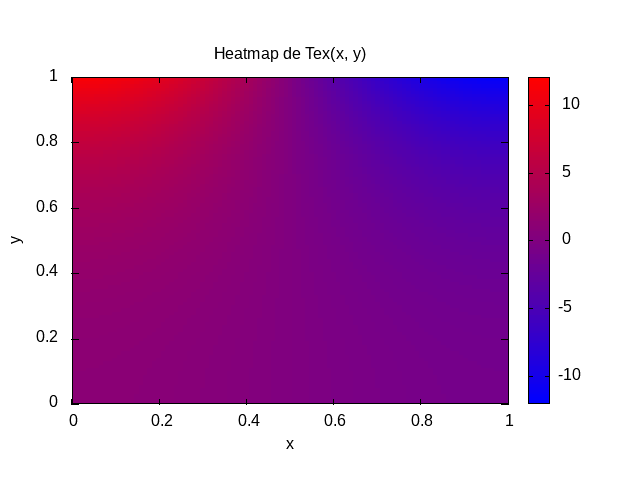
\includegraphics[scale=0.8]{newImages/Tex.png}
\]
Et voici la solution obtenue après calcul de la solution par la méthode d'Adomain:
\[
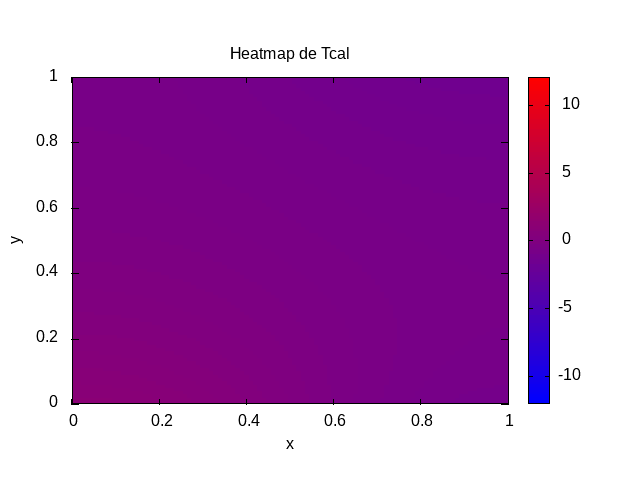
\includegraphics[scale=0.8]{newImages/Tcal_ado1.png}
\]
On voit alors que, à l'image des résulats pour le calcul de $f_3$, la solution calculée a tendance à atténuer les pics. On remarque de plus que le problème est clairement issue du calcul de $f_3^\alpha$. En effet, on voit bien que nos différence entre les deux schémas sont essentiellement localisées autour de $\Gamma_3$. Ailleurs, la solution calculeé semble relativement proche de la solution exacte.\\
On peut à présent vérifier nos dire en traçant la différence entre les deux solutions:
\[
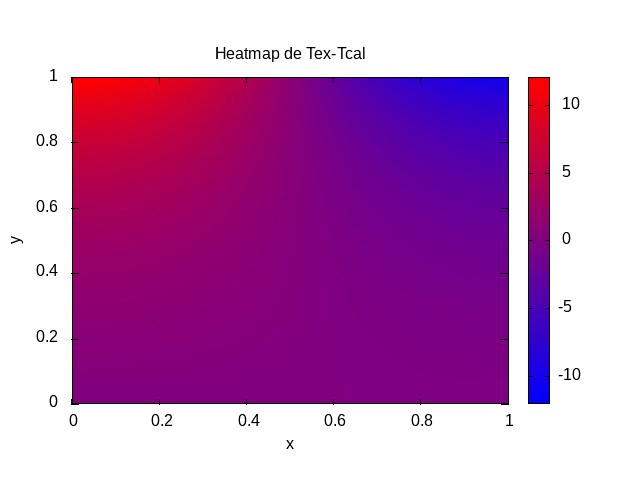
\includegraphics[scale=0.8]{newImages/Tex_Tcal_ado1.png}
\]
On voit alors que nos précédentes hypothèses sont vérifiées. En effet, on a une erreur qui est proche de 0 lorsque l'on regarde des points assez loin de $Gamma_3$. Cependant, on voit que plus l'on se rapproche de $Gamma_3$, plus les erreurs sont importantes. Comme nous l'avons dit précédemment, cela est du au fait que l'on a choisi un $f_3$ avec de forte variations sur un petit intervalle.\\
\\
Comme nous avons pu le voir, pour ce choix de $f_3$, la méthode d'Adomain n'est pas idéale. C'est pourquoi nous allons tenter d'appliquer la méthode d'Adomain d'une autre manière pour calculer un nouveau $f_3^\alpha$, qui, on l'espère sera une meilleure approximation de $f_3$.

\subsubsection{Méthode de décomposition d'Adomain v2}
La méthode d'approximation d'Adomain dans le cas général est :
$$
\left\{
    \begin{array}{ll}
        u_0(x) &= f(x) \neq 0 \\
         u_{n+1} &= \lambda\displaystyle\int_{0}^{L}k(x,t)u_n(t)dt
    \end{array}
\right.
$$
Donc pour $n\geq 2$ on a :
\begin{align*}
    u_{n}(x) &= \lambda\displaystyle\int_{0}^{L}k(x,s_1)u_{n-1}(s_1)\,ds_1 \\
        &= \lambda\displaystyle\int_{0}^{L}k(x,s_1)\left(\lambda \displaystyle\int_{0}^{L}k(s_1,s_2)u_{n-2}(s_2)ds_2\right)\,ds_1\\
        &=\lambda^{2}\displaystyle\int_{0}^{L}\displaystyle\int_{0}^{L}k(x,s_1)k(s_1,s_2)u_{n-2}(s_2)\,ds_2ds_1 \\
        &\vdots \\
        &= \lambda^n\displaystyle\int_{0}^{L}\cdots\displaystyle\int_{0}^{L} u_0(s_n)\prod_{i=1}^n k(s_{i-1},s_i)\,ds_n\cdots ds_1, \;\text{avec $s_0$=x}
        \end{align*}
        
Très clairement : $u_1(x)=\lambda\displaystyle\int_{0}^{L}k(x,t)u_0(t)dt=\lambda^{1} \displaystyle\int_{0}^{L} u_0(s_1)\prod_{i=1}^1 k(s_{i-1},s_i) ds_1 $\\
Donc on a, en posant $s_0=x$, $\forall n \geq 1$ :
$$u_{n}(x)= \lambda^n\displaystyle\int_{0}^{L}\cdots\displaystyle\int_{0}^{L} u_0(s_n)\prod_{i=1}^n k(s_{i-1},s_i)\,ds_n\cdots ds_1$$
Dans notre cas on a $\lambda = -\frac{1}{\alpha}$ et $u_0(x)=\frac{h(x)}{\alpha}$ \\
Donc par la méthode de décomposition d'Adomain où $f_3^\alpha(x)=\displaystyle\sum_{n=0}^{\infty}u_n(x)$, on a :
$$u_{n}(x)= -\left(\frac{-1}{\alpha}\right)^{n+1}\displaystyle\int_{0}^{L}\cdots\displaystyle\int_{0}^{L} h(s_n)\prod_{i=1}^n k(s_{i-1},s_i)\,ds_n\cdots ds_1$$
\\ \\
Maintenant nous souhaitons l'implémenter, cependant pour cela nous devons définir une fonction à n variables pour le calcul de chaque $u_n$, pour cela nous allons encore utiliser la quadrature de Gauss Legendre mais cette fois ci, en dimension n.\\
Le premier problème qui se pose à nous est comment, définir de manière itératives nos $s_0,s_1,...,s_n$,pour cela nous allons introduire le tableau d'entier $s[n+1]$. \\
Ce tableau est un tableau d'index allant de 0 à N-1, permet d'assigner une variable à un point de Gauss legendre.\\
exemple : pour s[n] donnée cela voudra dire que nous voulons calculer $$h(Xbis[s[n]])\prod_{i=1}^nk\left(Xbis[s[i-1]],Xbis[s[i]]\right)$$ \\
Ce qui permet de discrétiser notre espace de dimension n en le nombre de combinaisaison possible pour le tableau (en exeptant la première valeur de la boucle qui nous servira à representer le ).\\
Ce qui donne la création de la fonction :
$$Kn(s,x,n)=h(Xbis[s[n]])k\left(Xbis[x,Xbis[s[1]]\right)w[s[1]]\prod_{i=2}^n k\left(Xbis[s[i-1]],Xbis[s[i]]\right)w[s[i]] $$
(on sort le cas pour x, et on fait le produit tout de suite par les poids de Gauss Legendre pour pouvoir utiliser la quadrature plus tard)
et donc on aura :
$$U_n(x)\approx-\left(\frac{-1}{\alpha}\right)^{n+1}\left(\frac{L}{2}\right)^n\displaystyle\sum_{i_1=0}^{N-1}\cdots\displaystyle\sum_{i_n=0}^{N-1}Kn(s=\{0,i_1,...,i_n\},x,n)$$
Il ne nous reste plus qu'a créer une fonction les sommant pour de 1 à n, puis rajouté $\frac{h(x)}{\aplha}$, et nous avons notre $u(x)$ approché par la seconde méthode d'adomain.\\
Avant toute chose, on note que cette deuxième méthode d'approximation d'Adomain demande d'avantage de temps de calcul. En effet, on observe que la méthode tourne en $\mathcal{O}(N^n)$, où $n$ est le nombre d'itérations effectuée.\\
Cela la rendra bien moins efficace en terme de temps de calcul que la première version.
En effet, pour un x donnée ici 0.2, alpha , pour n=7 nous avons la première version de Adomain qui donne :
\[
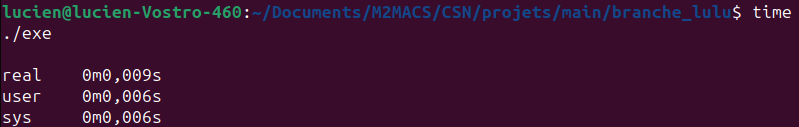
\includegraphics[scale=0.5]{newImages/time_ado1.png}
\]
tandis que la seconde version, pour les même donnée donne :
\[
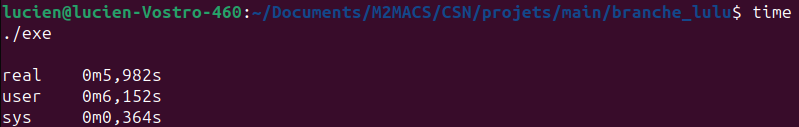
\includegraphics[scale=0.5]{newImages/time_ado2.png}
\]
Pour cette raison, nous allons diminuer le nombre d'itération sur n et prendre un pas plus grand. On prendra notamment un pas de 0,01 entre chaque point du maillage au lieu 0,001 pour la méthode précédente et on ne calculera cette fois que 3 itérations (au lieu de 5 pour la première méthode d'Adomain).
Maintenant nous voulons calculer le alpha optimal pour deuxième méthode d'Adomain, et nous obtenons :
\[
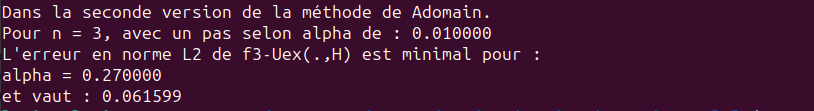
\includegraphics[scale=0.7]{newImages/err_adov2.png}
\]
À l'inverse de la première méthode, on arrive à trouver un alpha tel que l'erreur est de  l'ordre de $10^{-2}$, ce qui induit une bien meilleur approximation que notre première version de Adomain.\\
Cette différence n'est pas très logique, vu que ce sont deux version de la même méthode, nous avons essayé de trouver l'erreur qui pouvait se cacher dans l'un des deux codes et qui pouvait expliquer cela mais sans succés.\\ 

\\
On peut maintenant tracer la courbe des erreurs pour des $\alpha$ compris entre 0 et 10.
\[
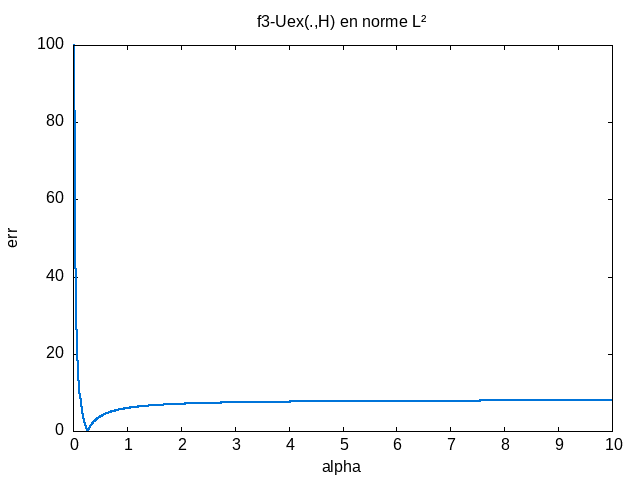
\includegraphics[scale=0.8]{newImages/T_err_alpha_adov2.png}
\]
On voit très bien le pic de convergence vers 0.27.\\
Maintenant on va tracer $f_3^\alpha$ approximer par  cette méthode :

\[
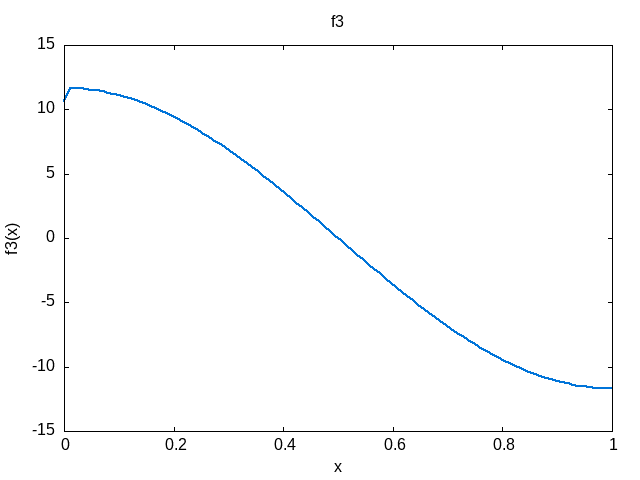
\includegraphics[scale=0.8]{newImages/f3_adov2.png}
\]
Nous pouvons voir que cela ressemble très fortement au tracé de $f_3 $ exacte, exepté au proche de x=0, où il y a une légère différence, surement du au fait que le n choisi n'est pas assez grand.// 
Maintenant, nous allons tracer la heatmap associée à notre solution calculée $\Tilde{T}^\alpha$ pour $L=H=1$ et $\alpha=0.27$ en utilisant la même expression que pour le calcul de $\Tilde{T}^\alpha$ par la première méthode d'Adomain:
\[
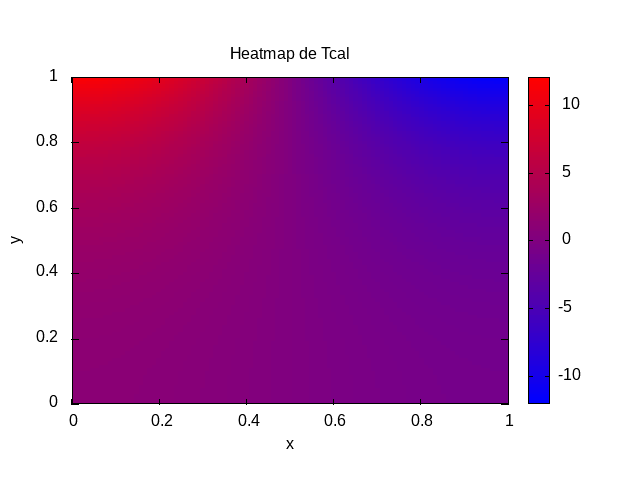
\includegraphics[scale=0.8]{newImages/Tcal_ado2.png}
\]
Pour rappel, on attendait une solution de la forme:
\[
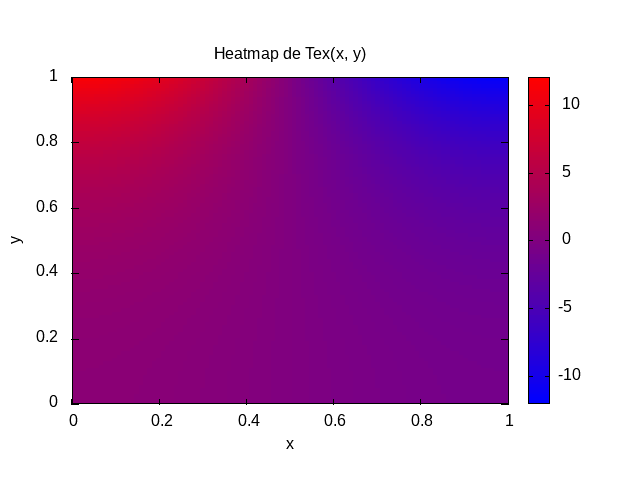
\includegraphics[scale=0.8]{newImages/Tex.png}
\]
On observe alors un résultat tout à fait semblable à la solution exacte.\\
On peut d'ailleurs maintenant tracer la heatmap des erreurs entre $\Tilde{T}^\alpha$ et $\Tilde{T}$.
\[
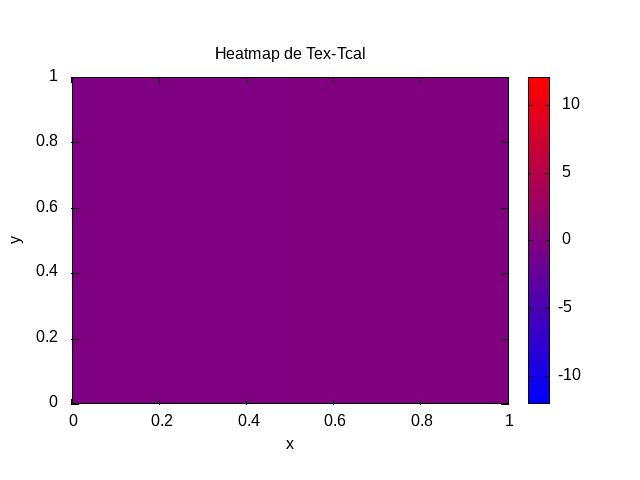
\includegraphics[scale=0.8]{newImages/Tex_Tcal_ado2.png}
\]
Cette heatmap nous montre que la seconde version de la méthode d'adomain permet de bine approximer T, cependant, le temps de calcul nécessaire n'est pas optimal, c'est pourquoi pour retrouver la frontière nous préfererons utiliser une autre méthode.
\subsection{Équation à noyaux séparables}
\subsubsection{Présentation de la méthode}
On a vu que la méthode d'Adomain n'était pas une méthode optimale pour approcher $f_3^{\alpha}$, soit car elle admet une erreur trop élevé, soit un temps de calcul bien trop long. On se propose donc d'approcher la fonction en utilisant la méthode des noyaux séparables.

On souhaîte toujours approcher $f_3$, l'inconnue de l'équation suivante:
\[
\alpha f_3(x) + \int_{0}^{L} k(x, t) f_3(t) dt = h(x)
\]

On remarque alors que, sachant que l'on a $\alpha >0$, cette équation peut-être équivalente à l'équation suivante:
\[
f_3(x) = \frac{h(x)}{\alpha}-\frac{1}{\alpha}\int_{0}^{L} k(x, t) f_3(t) dt
\]
soit:
\[
u(x)=f(x)+\theta\int_a^bk(x,t)u(t)dt
\]
Avec:
\[
\begin{enumerate}
    \item $u(x):=f_3(x)\\$
    \item $f(x):=\frac{h(x)}{\alpha}\\$
    \item $\theta :=\frac{-1}{\alpha}\\$
    \item $a:=0\\$
    \item $b:=L$
    \end{enumerate}
\]

L'hypothèse essentielle de la méthode des noyaux séparables sera alors la suivante. On suppose qu'il existe $n\in\mathbb{N}$, $n$ couples de fonctions $(\alpha_i,\beta_i)_{i\in\llbracket 1,n\rrbracket}$ (où $\forall i\in\llbracket 1,n\rrbracket$, $\alpha_i\in L^1$ et $\beta_i\in L^1$) tel que l'on peut écrire $k$ en le décomposant de la façon suivante.
\[ k(x; t) = \sum_{i=1}^{n} \alpha_i(x) \beta_i(t) \]

Vérifions donc que l'on peut écrire $k$ sous cette forme.\\
On rappelle l'expression de $k$:
\[
k(x, t) = \frac{1}{HL} + \frac{2\pi}{L^2} \sum_{m=1}^{n_k} \frac{m}{\sinh\left(\frac{m\pi H}{L}\right)} \cos\left(\frac{m\pi}{L}x\right)\cos\left(\frac{m\pi}{L}t\right)
\]
Alors, on voit qu'en choisissant $n=n_k+1$ et en prenant:
\[
\alpha_i(x)=
\left\{
\begin{align*}
    & \frac{1}{HL} & \text{     si }i=n\\
    & \frac{2\pi}{L^2}\frac{i}{\sinh\left(\frac{i\pi H}{L}\right)} \cos\left(\frac{i\pi}{L}x\right) & \text{      sinon}
\end{align*}
\]
et
\[
\beta_i(t)=
\left\{
\begin{align*}
    & 1 & \text{     si }i=n\\
    & \cos\left(\frac{i\pi}{L}t\right) & \text{      sinon}
\end{align*}
\]
On obtient bien 
\[ k(x; t) = \sum_{i=1}^{n} \alpha_i(x) \beta_i(t) \]

On peut alors réecrire notre équation sous la forme:
\[ u(x) = f(x) + \theta \int_{a}^{b} \sum_{i=1}^{n} \alpha_i(x) \beta_i(t) u(t) dt = f(x) + \theta \sum_{i=1}^{n} \alpha_i(x) \int_{a}^{b} \beta_i(t)u(t) dt \]
En posant
\[ c_i = \int_{a}^{b} \beta_i(t)u(t) dt; \quad i = 1, \ldots, n \]
On obtient
\[
\begin{equation}
    u(x) = f(x) + \theta \sum_{m=1}^{n} c_m \alpha_m(x)
\end{equation}
\]
où les \(c_i\) sont les constantes à déterminer. Pour ce faire, nous multiplions les deux membres de l'équation précédente par \(\alpha_m(x)\) et intégrons de \(a\) à \(b\) nous obtenons
\[ \int_{a}^{b} \alpha_m(x)u(x)dx = \int_{a}^{b} \alpha_m(x)f(x)dx + \theta \sum_{i=1}^{n} c_i \int_{a}^{b} \alpha_m(x) \alpha_i(x)dx \]
En utilisant les notations suivantes
\[ \int_{a}^{b} \alpha_m(x)f(x)dx = B_m; \quad \int_{a}^{b} \alpha_m(x) \alpha_i(x)dx = a_{mi} \]
la dernière équation devient
\[ c_m - \theta \sum_{i=1}^{n} c_i a_{mi} = B_m; \quad m = 1, \ldots, n \]

qui est un système d'équations linéaires de \(n\) inconnus de la forme :
\[ (I - \theta A) c = B \]
où \(I\) est la matrice identité et \(A = (a_{mi})_{1 \leq i,m \leq n}\) une matrice d'ordre \(n\); avec \(c\) et \(B\) des matrices colonnes.
Il suffit ensuite de résoudre ce système linéaire d'inconnue $c$. Dans notre cas, on a choisit de résoudre ce système en utilisant une décomposition LU de notre matrice $I - \theta A$. On obtient alors des valeurs pour $c$, que l'on peut réintégrer dans notre équation (1), pour obtenir une bonne approximation de $u$, et donc de $f_3$.

\subsubsection{Implémentation numérique}
Maintenant que l'on a explicité la méthode de résolution des noyaux séparables, on va pouvoir l'implémenter numériquement et juger de son efficacité.
On commence par calculer le $\alpha$ qui minimise l'erreur en norme $L^2$ entre $f_3$ et $f_3^\alpha$. On obtient:
\[
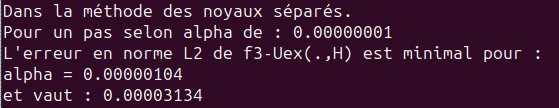
\includegraphics[scale=0.7]{Images/Capture d’écran du 2023-11-27 18-14-14.png}
\]
On en déduit donc que la méthode d'approximation des noyaux séparables est une bonne méthode d'approximation pour $f_3$. De plus, on remarque qu'elle approche  beaucoup mieux notre solution exacte que la méthode d'approximation d'Adomain version 1, et vu qu'elle ne demande que très peu de ressources au niveau du calcul, elle est bien plus performante que la méthode d'adomain en général.
Traçons maintenant l'évolution de l'erreur en fonction des $\alpha$. On obtient le graphique suivant:
\[
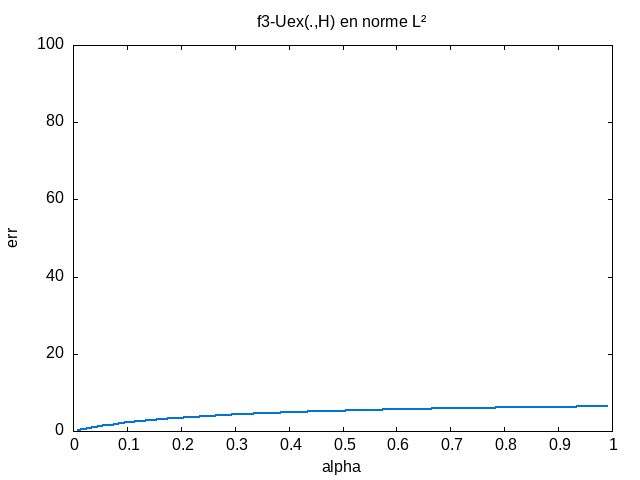
\includegraphics[scale=0.8]{Images/T_err_alpha_ker_sep.png}
\]
On voit alors bien que les erreurs sont moindre par rapport à la méthode d'Adomain, et que, de plus, l'erreur tend vers 0 lorsque $\alpha$ tend vers 0. Cela confirme donc nos hypothèses théoriques.

On peut à présent tracer la courbe de $f_3^\alpha$ calculée par la méthode des noyaux séparés:
\[
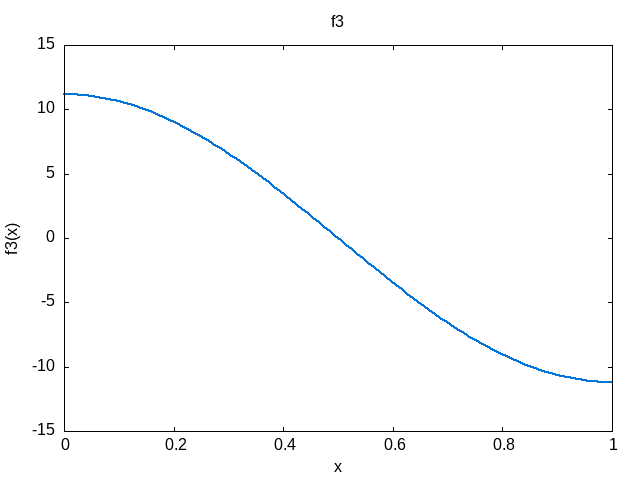
\includegraphics[scale=0.8]{Images/f3_ker_sep.png}
\]
alors que le tracé de $f_3$ est :
\[
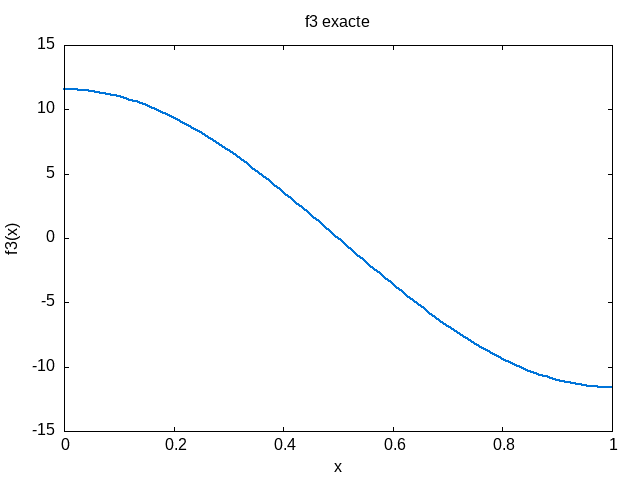
\includegraphics[scale=0.8]{newImages/f3_ex.png}
\]

On remarque que notre méthode des noyaux séparables à l'aire de parfaitement approximé la $f_3$\\
\\
Traçons maintenant notre solution $\Tilde{T}^\alpha$ que l'on détermine avec l'expression (1), pour $H=L=1$.
\[
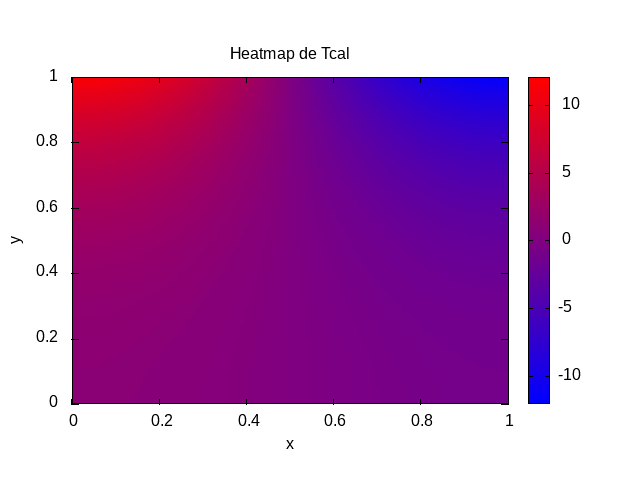
\includegraphics[scale=0.8]{newImages/Tcal_KS.png}
\]
Et on peut comparer avec la solution exacte définie par $\Tilde{T}(x,y)=\cos (\pi x)\cosh (\pi y)$ que l'on trace ci-dessous.
\[
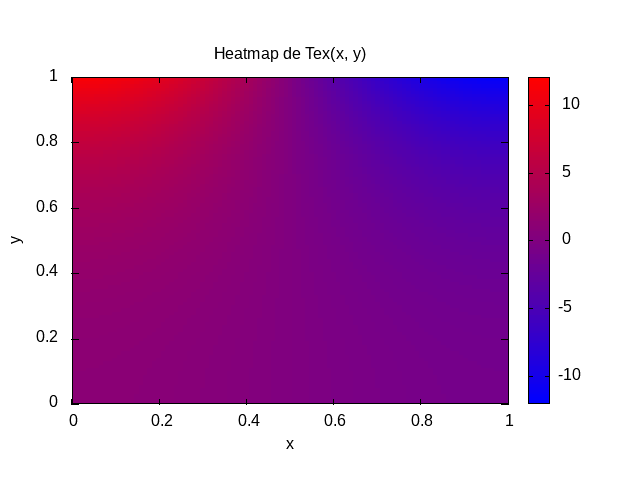
\includegraphics[scale=0.8]{newImages/Tex.png}
\]
On voit alors que, contrairement aux précédentes méthodes, et à l'instar de nos résultats pour le calcul de $f_3^\alpha$ par la méthode des noyaux séparables, la solution approchée $\Tilde{T}^\alpha$ est quasi-identique à la solution exacte $\Tilde{T}$. Cela nous confirme que la détermination d'une bonne approximation $f_3^\alpha$ est plus que déterminante pour résoudre ce problème. En effet, on voit que lorsque l'on trouve un $f_3^\alpha$ très proche $f_3$, derrière, on a également $\Tilde{T}^\alpha$ très proche de $\Tilde{T}$. La réciproque de ce postulat est d'ailleurs également vraie. En effet, on a vu dans nos deux méthodes d'Adomain qu'en obtenant des $f_3^\alpha$ approximatifs, on obtenait ensuite des $\Tilde{T}^\alpha$ approximatifs eux aussi.\\
\\
On peut maintenant confirmer la bon fonctionnement de notre méthode en traçant l'erreur entre $\Tilde{T}$ et $\Tilde{T}^\alpha$:
\[
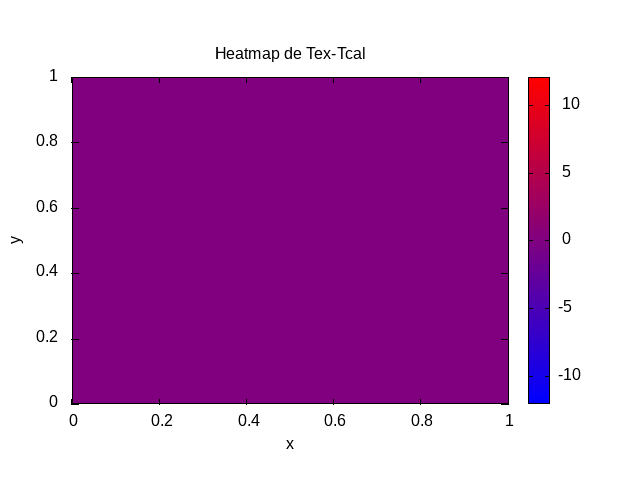
\includegraphics[scale=0.8]{newImages/Tex_Tcal_KS.png}
\]
Le tracer de cette erreur nous confirme donc bien que $\Tilde{T}^\alpha$ approche très bien $\Tilde{T}$. En effet, on voit que l'erreur est très proche de 0 sur tout l'espace $\lbrack 0,L\rbrack\times\lbrack 0,H\rbrack$.\\
\\
On en déduit donc que l'approximation par la méthode des noyaux séparables est une bien meilleure méthode d'approximation que celle d'Adomain dans le cas de notre fonction $f_3$. On pourra cependant émettre une limite quand à cette méthode car on remarque que si l'on avait pas pu dissocier $k$ en une somme de produit de fonctions à une variable, nous n'aurions pas pu appliquer cette méthode. Ainsi, selon l'expression de $k$ on pourra choisir d'utiliser plutôt la méthode d'approximation des noyaux séparables ou plutôt celle d'Adomain.
\subsection{Méthode des approximations successives}
\subsubsection{Présentation de la méthode}
La dernière métode par laquelle nous allons tenter d'approcher $f_3$ est la méthode des approximations successives. Cette méthode repose à nouveau sur le fait d'avoir une équation du type:
\[
\begin{equation}
    u(x)=f(x)+\lambda\int_a^bk(x,t)u(t)dt
\end{equation}
\]
On rappel alors à nouveau que dans notre cas, l'équation 
\[
\alpha f_3(x) + \int_{0}^{L} k(x, t) f_3(t) dt = h(x)
\]
peut être équivalente à l'équation précédente en définissant:
\[
\begin{enumerate}
    \item $u(x):=f_3(x)\\$
    \item $f(x):=\frac{h(x)}{\alpha}\\$
    \item $\lambda:=\frac{-1}{\alpha}\\$
    \item $a:=0\\$
    \item $b:=L$
    \end{enumerate}
\]

On va donc pouvoir appliquer la méthode des approximations successives pour approcher $f_3$.\\
Pour appliquer cette méthode, on a besoin de définir la suite $u_n$ suivante:
\[
\begin{cases}
u_0(x) = \text{une fonction arbitraire à valeur réelle.} \\
u_{n+1}(x) = f(x) + \lambda \int_{a}^{b} k(x; t) u_n(t) dt
\end{cases}
\]
La méthode repose alors sur le théorème suivant:
\[
\textit{Si \(f(x)\) est continue sur \([a; b]\) et \(k(x; t)\) est continu sur \([a; b] \times [a; b]\), alors la suite}
\]
\[
\textit{ \(u_n\) converge vers la solution de l'équation intégrale donnée.}
\]

\\
\\
\\
\\
On en déduit ainsi que l'équation (2), n'est autre que le passage à la limite de l'expression
\[
u_{n+1}(x) = f(x) + \theta \int_{a}^{b} k(x; t) u_n(t) dt
\]
Ainsi, la méthode des approximations successives consiste à implémenter cette suite le plus loin possible afin d'avoir une bonne approximation de la solution $u=f_3$.\\
Dans notre cas, on choisira comme fonction de départ, la foncton nulle.\\
Cependant, en changeant la fonction f dans le main, on peut avoir la méthode pour n'importe quelle fonctions.\\

Pour l'implémentation numérique cela ressemblera énormement à la première version de notre méthode d'Adomain.\\
Dans le sens où pour chaque $U_i$, i allant de 1 à n, nous allons les calculer sur les N points de Gauss Legendre(adapté à notre cas par changement de variable)  qui nous intéressent pour pouvoir l'intégrer par la suite, c'est à dire pour k de 1 à n, nous allons définir à chaque itérations N points i de 0à N-1:
$$U_{k+1}[Xbis[j]]=\frac{h(Xbis[j])}{alpha} + \displaystyle\sum_{i=0}^{N-1} k(Xbis[j],Xbis[i])U_k[Xbis[i]]$$
Nous initierons par f prise dans les valeur de Xbis[] pour U0, (bien sur nous ne travaillons que sur deux vecteur U et Ubis, que nous réfinissons à chaque itérations, correspondant à $U_{n+1}$ et $U_n$).
Et pour le dernier terme, nous ferons juste :
$$U_n[x]=\frac{h(x)}{alpha} + \displaystyle\sum_{i=0}^{N-1} k(x,Xbis[i])U_n[Xbis[i]]$$
Et nous renverrons le résultats obtenu.\\
Pour cette méthode nous allons chercher chercher son $\alpha$ optimal :
\[
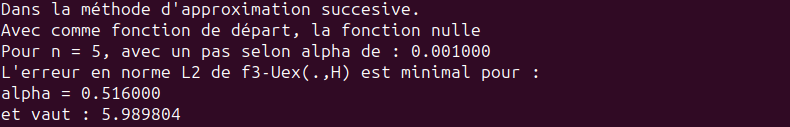
\includegraphics[scale=0.8]{Images/alpha_opt_AS.png}
\]
Nous allons ensuite tracer le graphe des erreurs en fonction de alpha :
\[
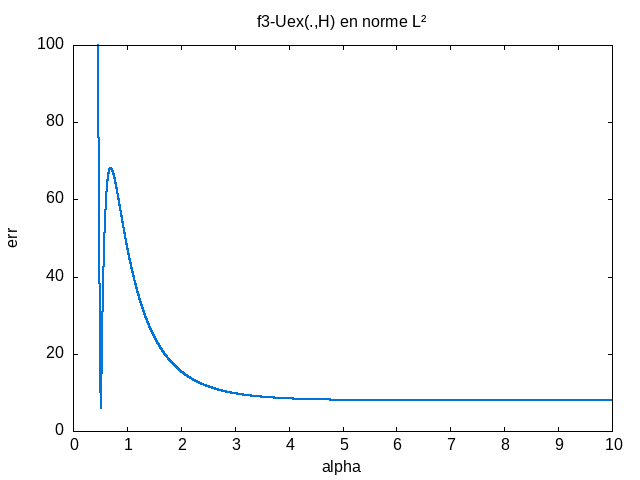
\includegraphics[scale=0.8]{Images/T_err_alpha_approx_succesive.png}
\]
On remarque bien le pic de convergence en 0.5
Et si on veut tracer le f3 correspondant, on obtient.
\[
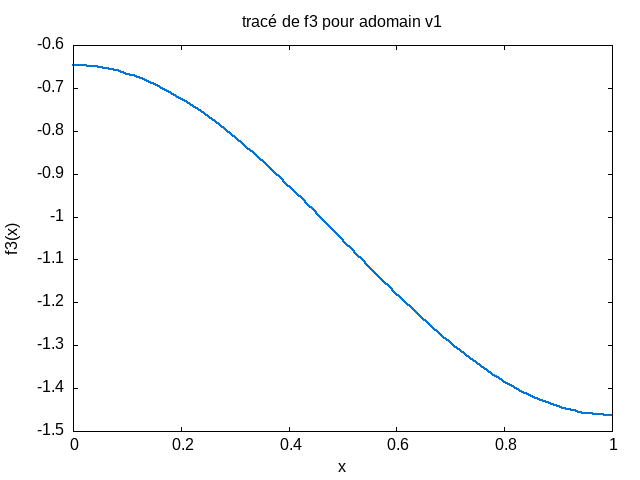
\includegraphics[scale=0.8]{newImages/f3_AS.png}
\]
Et la heatmap correspondante :
\[
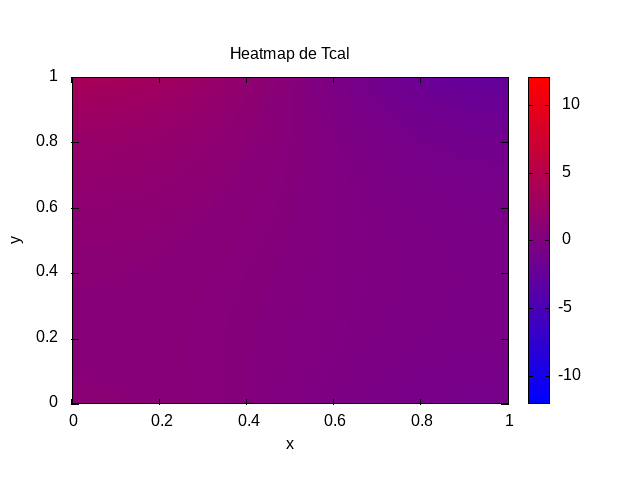
\includegraphics[scale=0.8]{newImages/Tcal_AS.png}
\]
on remarque cette aprpcohe ne converge pas très bien vers T(x,y), on va y préférer la méthode des nopyaux séparables.

\subsubsection{Implémentation numérique}
\subsection{Comparaison finale des $f_3^\alpha$}
Pour conclure sur la partie des méthodes, nous pouvons tracer un graphique qui regroupe les fonctions $f_3^\alpha$ pour chaque méthode, chacune associée à son $\alpha$ qui minimise l'erreur:
\[
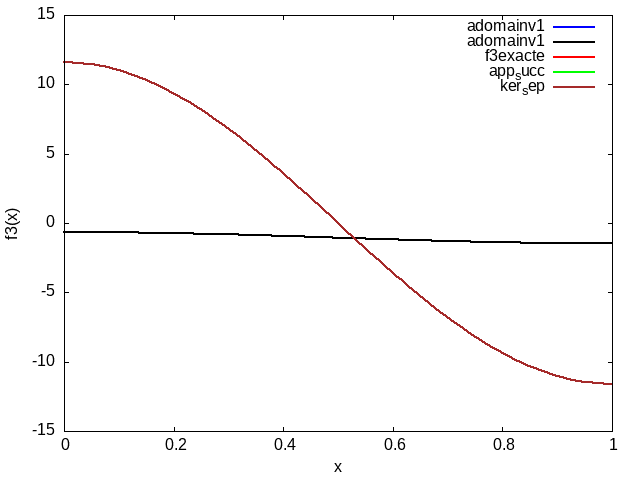
\includegraphics[scale=0.8]{newImages/f3_comparaison.png}
\]
Sur ce graphique, on peut voir que les courbes de $f_3$, $f_3^\alph$ associée à la méthode des noyaux séparables et $f_3^\alpha$ associée à la seconde méthode d'Adomain sont confondues entre elles tandis que les courbes de $f_3^\alpha$ associée à la métrhode des approximations successives et la courbe de $f_3^\alpha$ associée à la première méthode d'Adomain sont également confondues entre elles.\\
Ce schéma illustre bien la situation de chacune de nos méthode. En effet, on voit que les deux méthodes qui marchent le mieux sont très efficaces tandis que les 2 méthodes qui marchent moins bien sont relativement loin de la courbe de $f_3$, tout en restant confondues. Sachant que l'on a repris une partie du code de la première méthode d'Adomain pour implémenter notre méthode des approximations successives, on suppose que l'on a laissé traîner une erreur dans notre première version d'Adomain qui se répercute sur notre méthode d'approximations successives. Cela explique notamment le fait que l'on obtienne le même $\alpha$ minimisant pour les deux méthodes, la même erreur sur $\Gamma_3$ et le fait que les courbes soit confondues.
\section{Trouver $\Gamma$}
\subsection{L'algorithme de Newton}
On veut maintenant trouver une approximation de $\Gamma$ qui est également inconnu. Pour cela, on se sert d'un  $\Gamma$ factuel associé à $u_{ex}(x,y)=cos(\pi x)\cosh \left(y\right)$ et, comme pour la détermination de $f_0$, $q_0$ et $f_3$ on pourra se servir de ce $\Gamma$ factuel afin d'obtenir $T_0$.
On pose :
\[
\Gamma=\left\{ (x;y)\in\mathbb{R}^2|y=0,7\right\}
\]
Ce qui donne:
\[
T_0(x)=u_{ex}(x,f(x))=\cos(\pi x)\cosh \left(0,7\right)
\]
avec $f(x)=0,7$ la fonction qui définit $\Gamma$\\
\\
\\
\underline{NB:} Ici, on ne s'interresse qu'à la détermination de $\Gamma^\alpha$ associé à la méthode des noyaux séparables car on a vu qu'il s'agissait de la méthode qui convergeait le mieux, cependant, dans notre code on calcule $\Gamma^\alpha$ pour toute les méthodes. On notera également que, dans notre code, pour tester nos approximations sur différents $\Gamma$, on a choisi différentes valeur de $f(x)$. En locurrence, on choisit $f(x)=0,7$ pour le $\Gamma^\alpha$ associé à la méthode des noyaux séparables et on choisit $f(x)=x$ pour toute les autres méthodes.\\
\\

Maintenant que nous avons définit notre $T_0$, nous allons pouvoir essayer de retrouver $\Gamma$. Or nous savons que rechercher $\Gamma$ revient à chercher les $y$ tels que l'équation suivante soit vraie $\forall x \in \lbrack 0;L\rbrack$:
\[
T(x;y)-T_0(x)=0
\]
Comme $T(x;y)-T_0(x)$ est $\mathcal{C}^1(\mathbb{R}^2)$, on a juste à implémenter un algorithme de Newton pour obtenir le 0 de cette fonction lorsque l'on fixe $x$.
Ainsi, pour chaque $x\in\rbrack 0,L\lbrack$, on détermine un point $y^\alpha$ associé.
\subsection{Résultat numérique}
Maintenant que l'on a implémenter notre méthode, on peut observer les résultats que l'on obtient:

\[
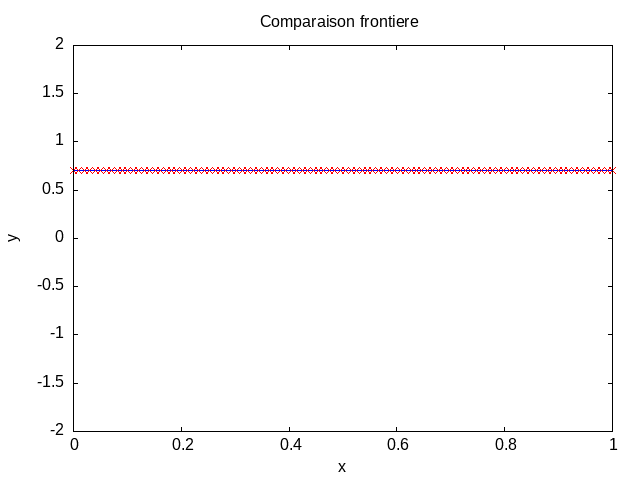
\includegraphics[scale=0.8]{newImages/comparaison_frontiere.png}
\]
On voit alors que la courbe de nos $y^\alpha$, ici représentés par les croix rouges suit parfaitement la courbe de notre $\Gamma$ avec $f(x)=0,7$. Cela nous montre donc à nouveau à quel point la méthode des noyaux séparables est efficace pour résoudre notre problème.\\
\\
Etant donné le graphique ci-dessus nous pouvons considérer que nous avons résolu le problème principal qui était de trouver une méthode capable d'approcher correctement la solution exacte $T$ avec son $f_3$ associé, ainsi que la frontière libre $\Gamma$.
\section{Conclusion}
En effet, on a vu que la méthode des noyaux séparables convergeait très bien lorque $\alpha\to 0$. De plus elle permet d'avoir une bonne très bonne approximation de $f_3$, $T$ et $\Gamma$. On notera cependant que la méthode possède un inconvéniant majeur: elle n'est applicable que si $k$ est décomposable en une somme finie de produit de fonctions à une variable. Si cette condition ne peut être vérifié, on s'orientera alors plutôt vers l'utilisation d'une méthode de type Adomain par exemple. La deuxième proposition de méthode d'approximation d'Adomain est d'ailleurs très interressante malgré le fait qu'elle ait un coût de calcul très élevé par rapport à la méthode d'approximation des noyaux séparables. La première méthode d'Adomain et la méthode des approximations successives sont quant à elle a éviter. En effet, elle semblent ne pas converger aussi efficacement que les deux autres méthodes. C'est du moins la conclusion que l'on tire, malgré notre suspicion d'une petite coquille dans notre programmation de ces-dernières.
\end{document}